% !TEX TS-program = pdflatex
% !TEX encoding = UTF-8 Unicode

% TO COMPILE: lmake (animal scrifices may be necessary)
%%%%%%%%%%%%%%%%%%%%%%%%%%%%%%%%%%%%%%%%%%%%%%%%%%%%%%%%%%%%%%%%%%%%%%%%%%
%																							                           %
%				                         PREAMBLE      							             %
%                                                                        %
%%%%%%%%%%%%%%%%%%%%%%%%%%%%%%%%%%%%%%%%%%%%%%%%%%%%%%%%%%%%%%%%%%%%%%%%%%
\documentclass[compress]{beamer}

\mode<presentation>
{
  \usetheme{Frankfurt}
  \usecolortheme{crane}
  \setbeamercovered{transparent}
}

% Package Setup
%%%%%%%%%%%%%%%%%%%%%%%%%%%%%%%%%%%%%%%%%%%%%%%%%%%%%%%%%%%%%%%%%%%%%%%%%%
%                                                                        %
%                                 PREAMBLE                               %
%                                                                        %
%%%%%%%%%%%%%%%%%%%%%%%%%%%%%%%%%%%%%%%%%%%%%%%%%%%%%%%%%%%%%%%%%%%%%%%%%%

%% PACKAGES
\usepackage[]{lineno}
\usepackage{fancyvrb}
%\linenumbers
\usepackage{amsmath}
\usepackage{microtype}
\usepackage{algorithmic}

%% GRAPHICS RELATED
\usepackage{graphicx}
\usepackage[outdir=./tmp/]{epstopdf}
\graphicspath{{../images/}{./}{./tmp/}}
\DeclareGraphicsExtensions{.eps, .pdf, .jpeg, .png}

%% CAPTION SETUP
\usepackage{float}
\usepackage[font=footnotesize]{caption}
\usepackage[font=small]{subcaption}
\captionsetup{belowskip=12pt,aboveskip=4pt}

%% BEAMER
\usepackage{multicol}
\usepackage{multirow}
\usepackage{array}				% Table Stuff
\usepackage{arydshln}
\usepackage{rotating}

%% BIBLIOGRAPHY
\bibliographystyle{ieeetr}

%% UNITS
\usepackage{siunitx}

%% EQUATIONS
%\numberwithin{equation}{section}

%%%%%%%%%%%%%%%%%%%%%%%%%%%%%%%%%%%%%%%%%%%%%%%%%%%%%%%%%%%%%%%%%%%%%%%%%%%
%                                                                         %
%                             Listing Setup                               %
%                                                                         %
%%%%%%%%%%%%%%%%%%%%%%%%%%%%%%%%%%%%%%%%%%%%%%%%%%%%%%%%%%%%%%%%%%%%%%%%%%%
\usepackage{listings}
\lstset{ %
    language=C++,
    basicstyle=\footnotesize\ttfamily,
    numbers=left,
    numberstyle=\tiny\color{gray},
    stepnumber=2,
    numbersep=5pt,
    backgroundcolor=\color{white},
    showspaces=false,
    showstringspaces=false,
    showtabs=false,
    frame=single,
    rulecolor=\color{black},
    tabsize=2,
    breaklines=true,
    breakatwhitespace=false,
    title=\lstname,
    keywordstyle=\color{blue},
    commentstyle=\color{OliveGreen},
    stringstyle=\color{orange}
}
\DeclareCaptionFont{white}{\color{white}}
\DeclareCaptionFormat{listing}{\colorbox[cmyk]{0.43, 0.35, 0.35, 0.01}{\parbox{\dimexpr\textwidth-2\fboxsep\relax}{#1#2#3}}}
\captionsetup[lstlisting]{format=listing,labelfont=white,textfont=white,singlelinecheck=false,margin=0pt,font={bf,footnotesize}}
%\lstnewenvironment{code}[1][]%
%{ \noindent\minipage{\linewidth}
%	\lstset{#1}
%}
%{\endminipage}
%% USER COMMANDS
\usepackage{isotope}
\newcommand{\iso}{\isotope}
\newcommand{\figurewidth}{\textwidth}
\newcommand{\micron}{$\mu$m}



% Preamble / Frst Size
%\setbeamersize{text margin left=5mm, text margin right 5mm}
\title[ANS 2013] {Characterization and Simulation of Thin Polymeric Films for Portal Monitors}
\author[] {
    Matthew Urffer\inst{1} \and 
    R. Uppal \inst{2} \and 
    A.Mabe \inst{3}  \and
    D. Penumadu \inst{2} \and
    L. F. Miller \inst{1}
}
\institute[University of Tennessee] { 
  \inst{1}%
  Department of Nuclear Engineering,
  University of Tennessee, Knoxville, TN
    \\
    \inst{2}
  Department of Civil Engineering,
  University of Tennessee, Knoxville, TN
  \\
  \inst{3}
  Department of Chemistry,
  University of Tennessee, Knoxville, TN

}

\date[] {June 19, 2013}
\pgfdeclareimage[height=0.5cm]{university-logo}{../images/utwordmarkhorz.png}
\logo{\pgfuseimage{university-logo}}

\begin{document}

\begin{frame}[plain]
  \titlepage
  \tiny
    \begin{center}
\centering{Financial support from the Domestic Nuclear Detection Office (DNDO) through Award No. 003387891 is gratefully acknowledged. 
  Any opinions, findings, and conclusions or recommendations expressed in this material are those of the presenter and do not necessarily reflect the views of DNDO.}
  \end{center}
\end{frame}

\begin{frame}{Talk Outline}
  \tableofcontents
\end{frame}


%%%%%%%%%%%%%%%%%%%%%%%%%%%%%%%%%%%%%%%%%%%%%%%%%%%%%%%%%%%%%%%%%%%%%%%%%%
%                                                                        %
%                            INTRODUCTION                                %
%                                                                        %
%%%%%%%%%%%%%%%%%%%%%%%%%%%%%%%%%%%%%%%%%%%%%%%%%%%%%%%%%%%%%%%%%%%%%%%%%%
\section{Introduction}

A supervised machine learning problem is one which a learning algorithm is presented a set of training data and attempts to find an unknown function which maps the training values to the correct answer.
Typically the training set, denoted $S$, is a set of the form $\left \{ (\vec{x}_1,y_1), (\vec{x}_2,y_2), \dots, (\vec{x}_n,y_n) \right \}$ where $\vec{x}_i$ is vector of some features of the problem.
Examples of problem features include discrete or real valued items such as height, weight, age, zip code, grade point average, starting salary, and telephone number (as just a few)  which might make up the features of a person.
The $y_i$ are the class of the training feature $\vec{x}_i$ belongs to; these might be University of Tennessee students or Carnegie Mellon students.
In this examples students with a zip code of 15213 are likely to be Tartans, while students with a zip code of 37916 are like to be Volunteers.
The challenge arises from examples have overlapping features; for example this author as a former Tartan and current Vol would be difficult to classify by zip code.
The learning algorithms job is then to find a hypothesis $h$ that correctly classifies a student as a Volunteer of Tartan based on the features provided.
This learning process can then be defined as finding the hypothesis that has the least error (incorrect classifications) on the training data set while extending to examples outside of the training space.

\subsection{Support Vector Machines}
Support Vector Machines (SVM) are a supervised learning technique in which hyperplanes are constructed in a high dimensional space to which the features are mapped.
SVMs find the hyperplanes that are the farthest away from all of mapped features in order to provide excellent training performance while still maintaining the ability to generalize to new instances; i.e. SVMs are maximal margin classifiers.
For a binary classification the decision function of the SVM is the dot product of the weight vector and the training example in the feature space added to a bias vector as shown in Equation \ref{eq:BCSVM}.
\begin{equation}
\label{eq:BCSVM}
f \left ( \vec{x} \right ) = \left \langle \vec{w} \phi(\vec{x}) \right \rangle + \vec{b}
\end{equation}
where $\phi(\vec{x})$ is a mapping to the higher dimensional space.
The SVM is then learning the optimal values of the weight vector $\vec{w}$ and the basis $\vec{b}$.

The radial basis function (Equation \ref{eq:RBF}) is a common kernel function used to map the input vector $\vec{x}$ into a higher dimension.
\begin{equation}
\label{eq:RBF}
k \left ( \vec{x}_i , \vec{x}_j \right ) = exp \left ( - \frac{\left \| \vec{x}_i - \vec{x}_j \right \|}{2\sigma^2} \right ) 
\end{equation}
The maximal margin is ensured by minimizing:
\begin{equation}
\label{eq:Min}
g(\vec{w},\eta) = \frac{1}{2} \left \| \vec{w} \right \| + C \sum_{i=1}^N \zeta_i
\end{equation}
subject to:
\begin{equation}
\label{eq:Constraint}
y_i( \left \langle \vec{w},\phi(\vec{x}) \right \rangle + b ) \ge 1-\zeta_i, ~~~\zeta_i \ge 0
\end{equation}
where $\zeta_i$ is the $i$th slack variable and C is the regularization parameter \cite{li_adaboost_2008}.
This problem can be translated  in to the Wolfe dual form, which can be solved with quadratic programing \cite{li_adaboost_2008}.

\subsection{Boosting}
Unbalanced data sets (data sets in which a majority of the values come from one class, see Figure \ref{fig:ClassDist}) are difficult for classification schemes to learn because the minority class is not well represented and tends to be thought as noise for the classifier.
Often classifiers are trained from unbalanced data sets by artificially balancing the data set by sampling techniques; i.e. up-sampling (sampling more from the minority class) and down-sampling (sampling less from the majority class).
Boosting is an ensemble learning method in which a set of weights is maintained over the training samples and adaptively adjusted after each training iteration according to the ones that are misclassified \cite{li_adaboost_2008}.
Given an individual classifier $h$, an ensemble of classifiers can be constructed of a set of individual classifiers, $H={h_1, h_2,\dot, h_n}$.
By maintaining a weight distribution over all of the training examples, these weights could be updated to emphasize the training examples that are misclassified incorrectly.  These incorrectly classified examples could then be learned in a refinement of the classifier or by training adding a new classifier to the ensemble with the new weights.
Performance of the ensemble is enhanced as long as the individual classifiers are weak and have uncorrelated errors as when any single classifier is incorrect the other classifiers in the ensemble might correctly classify the example.
\begin{figure*}[ht!]
	\centering
	\begin{subfigure}[b]{0.3\textwidth}
		\centering
		\includegraphics[width=\textwidth]{Liver_ClassDist}
        \caption{Liver}
	\end{subfigure}%
	~
	\begin{subfigure}[b]{0.3\textwidth}
		\centering
		\includegraphics[width=\textwidth]{Glass_ClassDist}
        \caption{Glass}
	\end{subfigure}	
    ~
	\begin{subfigure}[b]{0.3\textwidth}
		\centering
		\includegraphics[width=\textwidth]{Vowel_ClassDist}
        \caption{Vowel}
	\end{subfigure}%
	\caption{Distribution of Class Data}
	\label{fig:ClassDist}
\end{figure*}

\section{Energy Deposition}
\subsection{Motivation}
%%%%%%%%%%%%%%%%%%%%%%%%%%%%%%%%%%%%%%%%%%%%%%%%%%%%%%%%%%%%%%%%%%%%%%%%%%
\begin{frame}{Single Collision Energy Loss}
How much energy does an electron lose in a collision?
  \newtheorem{thm1}{Single Collision Energy Loss Definition}
  \begin{thm1}<1->
    \small
    Interaction of an electron of kinetic energy E with water can be described by the probability $N(E,E')dE$ that it loses an amount of energy between $E'$ and $E'+dE$
  \end{thm1}
  \begin{itemize}
    \item $N(E,E')$ is the single collision spectrum of $E$
    \item $N(E,E')$ is a normalized probability function
  \end{itemize}
\end{frame}
%%%%%%%%%%%%%%%%%%%%%%%%%%%%%%%%%%%%%%%%%%%%%%%%%%%%%%%%%%%%%%%%%%%%%%%%%%
\begin{frame}[fragile]{Motivation}
  Secondary Electron Range Calculations:
  \begin{itemize}
    \item Low energy, high fidelity low energy electron transport needed for gamma discrimination simulation
    \item GEANT4 (with \verb+G4DNAPhysics+) provide the ability to simulate low energy electron interactions
    \item Ability to validate GEANT4 simulation
  \end{itemize}
  Neturon - Photon Discrimination:
  \begin{itemize}
    \item Secondary electrons from gamma interactions will have a higher energy than reaction products from neutorn interactions
    \item Higher energies imply a partial energy deposition, thus ability for pulse height discrimination
  \end{itemize}
\end{frame}
%%%%%%%%%%%%%%%%%%%%%%%%%%%%%%%%%%%%%%%%%%%%%%%%%%%%%%%%%%%%%%%%%%%%%%%%%%
\begin{frame}{Project Goal}
  \centering
  \begin{itemize}
    \item Validate GEANT4 simulation method by reproducing single collision energy loss spectra
    \item Apply this simulation to energy deposition in films
  \end{itemize}
  \begin{figure}
    \includegraphics[width=0.6\textwidth]{Turner_Fig2_SingleCollisionELoss}
  \end{figure}
  \flushleft
  \small
  Example:
  \begin{itemize}
    \tiny
    \item For \SI{10}{\keV}, the average value of the single collision energy loss between \SI{45}{\keV} to \SI{50}{\keV} is 0.1 $\text{eV}^{-1}$
    \item Interval is \SI{5}{\keV}, so 5\% chance that a \SI{10}{\keV} electron in water has an energy loss between \SI{45}{\keV} and \SI{50}{\keV} in it's first collision
  \end{itemize}
\end{frame}
%%%%%%%%%%%%%%%%%%%%%%%%%%%%%%%%%%%%%%%%%%%%%%%%%%%%%%%%%%%%%%%%%%%%%%%%%%
\begin{frame}{Monte Carlo Simulation Modeling}
Why Monte Carlo Simulation?
\begin{itemize}
  \item Can model the physical event
  \item Analytical solutions are hard
\end{itemize}
Why GEANT4?
\begin{itemize}
  \item Develop familarity with the toolkit
  \item GEANT4 has the ability to model low energy electrons
  \item GEANT4 has the ability to model light transport
\end{itemize}
\centering
The single collsion energy loss is a simple simulation with all of the energy transfer componenets necessary for detailed detector energy depostion.
\end{frame}
%%%%%%%%%%%%%%%%%%%%%%%%%%%%%%%%%%%%%%%%%%%%%%%%%%%%%%%%%%%%%%%%%%%%%%%%%%
%                                                                        %
%                                METHODS                                 %
%                                                                        %
%%%%%%%%%%%%%%%%%%%%%%%%%%%%%%%%%%%%%%%%%%%%%%%%%%%%%%%%%%%%%%%%%%%%%%%%%%
\section{Methods}
\subsection{GEANT4}
\begin{frame}[fragile]{GEANT4 Introduction}
What GEANT4 is:
\begin{itemize}
  \small
  \item \href{geant4.cern.ch}{geant4.cern.ch}
  \item Free software package for the simulation of the passage of particles through matter
  \item Essentially a collection of tools for geometry, materials, physics models, events and digitization, visualizations $\dots$
  \item Maintained by the CERN community, widely used in physics
\end{itemize}
What GEANT4 is not:
\begin{itemize}
  \small
  \item For the timid
  \begin{itemize}
    \item Users are responsible for correctly implementing their own physics
    \item Users are responsible for correctly implementing their own analysis
  \end{itemize}
  \item Stagnant - major release are still occurring
\end{itemize}
\end{frame}
%%%%%%%%%%%%%%%%%%%%%%%%%%%%%%%%%%%%%%%%%%%%%%%%%%%%%%%%%%%%%%%%%%%%%%%%%%
\begin{frame}[fragile]{GEANT4 Microdose Models}
\verb+G4DNAPhyscis+, \href{geant4-dna.in2p3.fr}{geant4-dna.in2p3.fr/index.html}
  \begin{itemize}
    \item A microdose model for modeling early biological damage by ionizing radiation on the DNA scale
    \item Electron interactions include: elastic scattering (\SI{7.4}{\eV}), electronic excitation (\SI{9}{\eV}), ionization (\SI{11}{\eV}), vibrational excitation (\SI{2}{\eV})
    \item Similar methods exist for the protons, alphas
    \item Only material defined is \verb+G4_WATER+ (NIST based)
  \end{itemize}
\end{frame}
%%%%%%%%%%%%%%%%%%%%%%%%%%%%%%%%%%%%%%%%%%%%%%%%%%%%%%%%%%%%%%%%%%%%%%%%%%
\begin{frame}[fragile]{Implemented Simulation}
  Single Collision Energy Loss:
  \begin{itemize}
     \item Electrons shot into a cube of water
     \item Initial events chosen by a particle gun
     \item Verbose tracking for first change in energy, in addition to binning on this value through ROOT
  \end{itemize}
  Energy Deposition in Thin Polymers:
  \begin{itemize}
    \item \SI{0.25}{\eV} neutrons and \iso[60]{Co} photons shot into \iso[6]{LiF} loaded polymer
    \item Energy deposition calculated for each event, binned over a run
  \end{itemize}
\end{frame}
%%%%%%%%%%%%%%%%%%%%%%%%%%%%%%%%%%%%%%%%%%%%%%%%%%%%%%%%%%%%%%%%%%%%%%%%%%
%                                                                        %
%                               RESULTS                                  %
%                                                                        %
%%%%%%%%%%%%%%%%%%%%%%%%%%%%%%%%%%%%%%%%%%%%%%%%%%%%%%%%%%%%%%%%%%%%%%%%%%
\section{Results}
\subsection{Single Collision Validation Results}
\begin{frame}{GEANT4 Single Collision Energy Loss}
  \begin{figure}
    \includegraphics[width=0.75\textwidth]{SingleCollisionEnergyLoss_300bins}
  \end{figure}
\end{frame}
\begin{frame}{Comparison to Turner}
  \begin{columns}[onlytextwidth]
    \begin{column}{0.45\textwidth}
      \begin{figure}
        \includegraphics[width=\textwidth]{Turner_Fig2_SingleCollisionELoss}
        \caption{Tuner Spectrum}
      \end{figure}
    \end{column}
    \begin{column}{0.45\textwidth}
      \begin{figure}
        \includegraphics[width=\textwidth]{SingleCollisionEnergyLoss_300bins}
        \caption{GEANT4 Simulated Spectrum}
    \end{figure}
    \end{column}
  \end{columns}
\vspace{2mm}
Discrepancies are in the resolution of cross section data
\end{frame}
\subsection{Energy Deposition}
\begin{frame}{Comparison to Measured Spectra}
  \begin{columns}
    \begin{column}{0.45\textwidth}
      \centering
      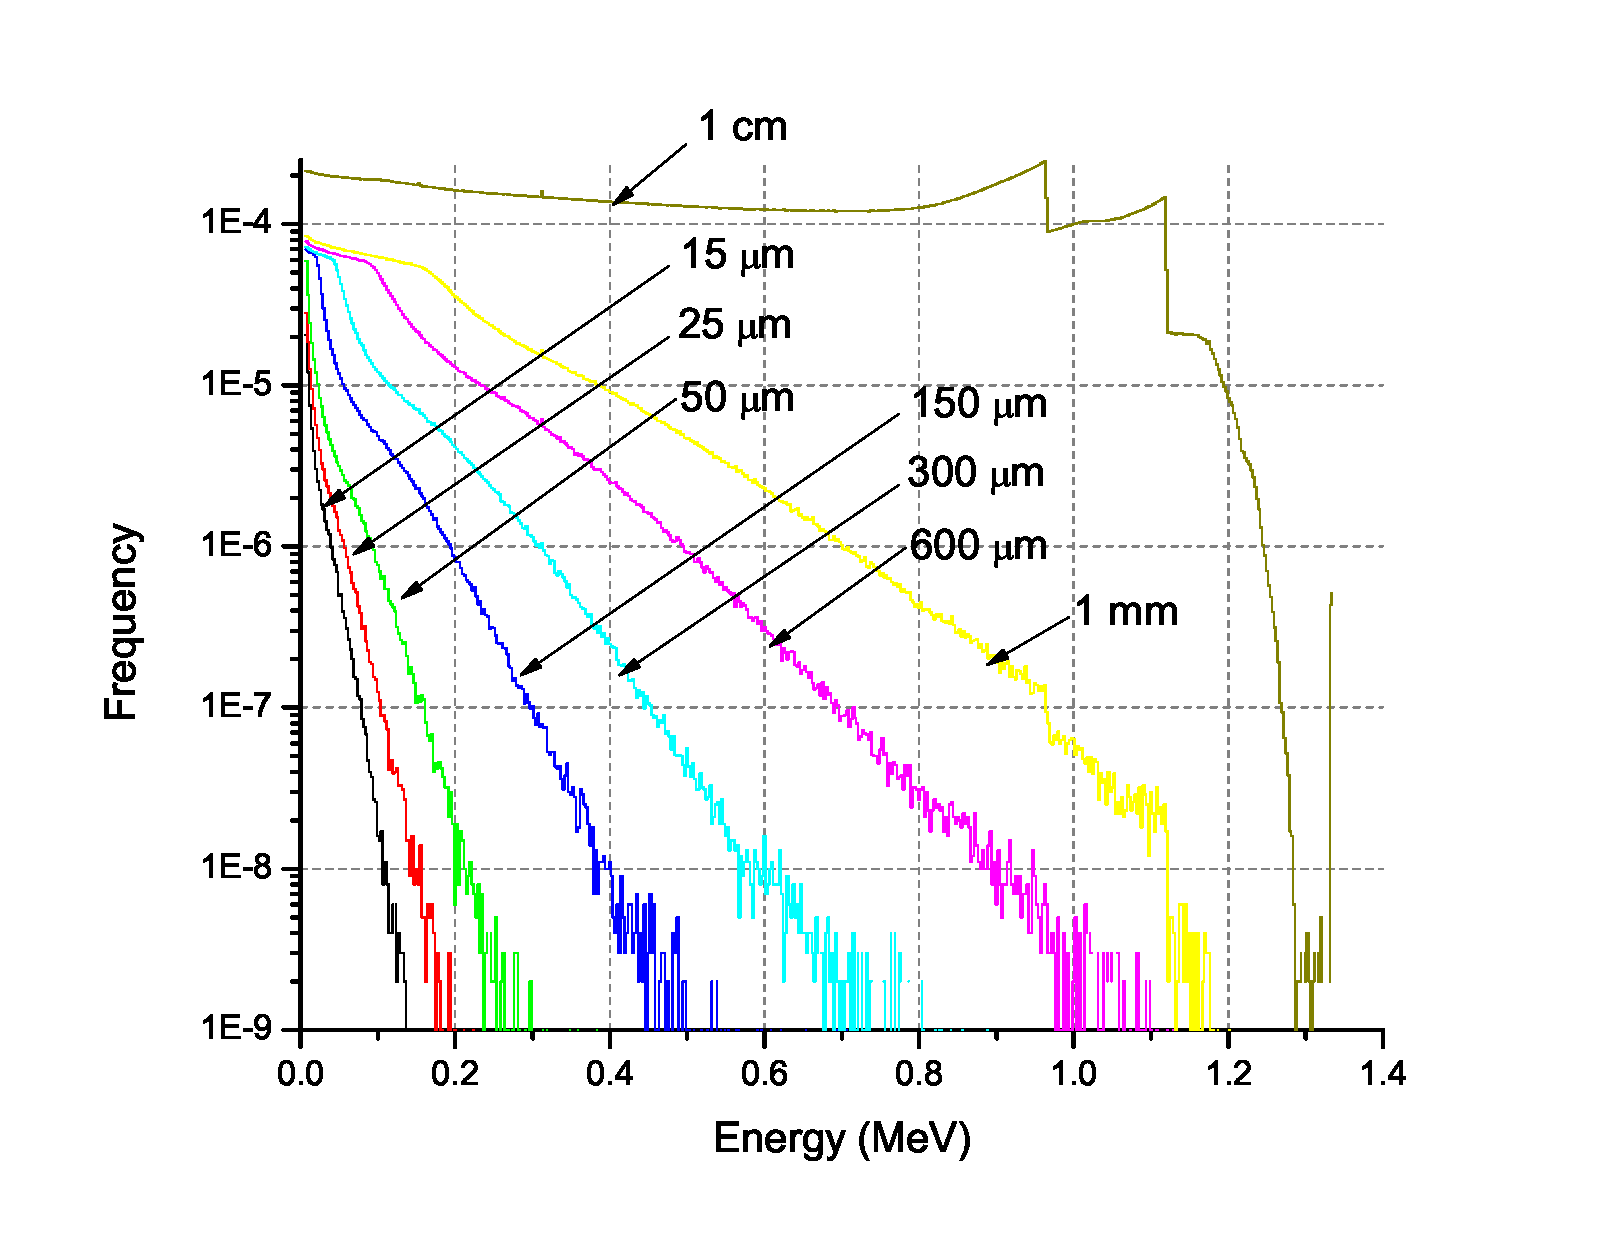
\includegraphics[width=\textwidth]{PS_EDepSim_Co60}

     GEANT4 Simulated Energy Deposition
    \end{column}
    \begin{column}{0.45\textwidth}
      \centering
      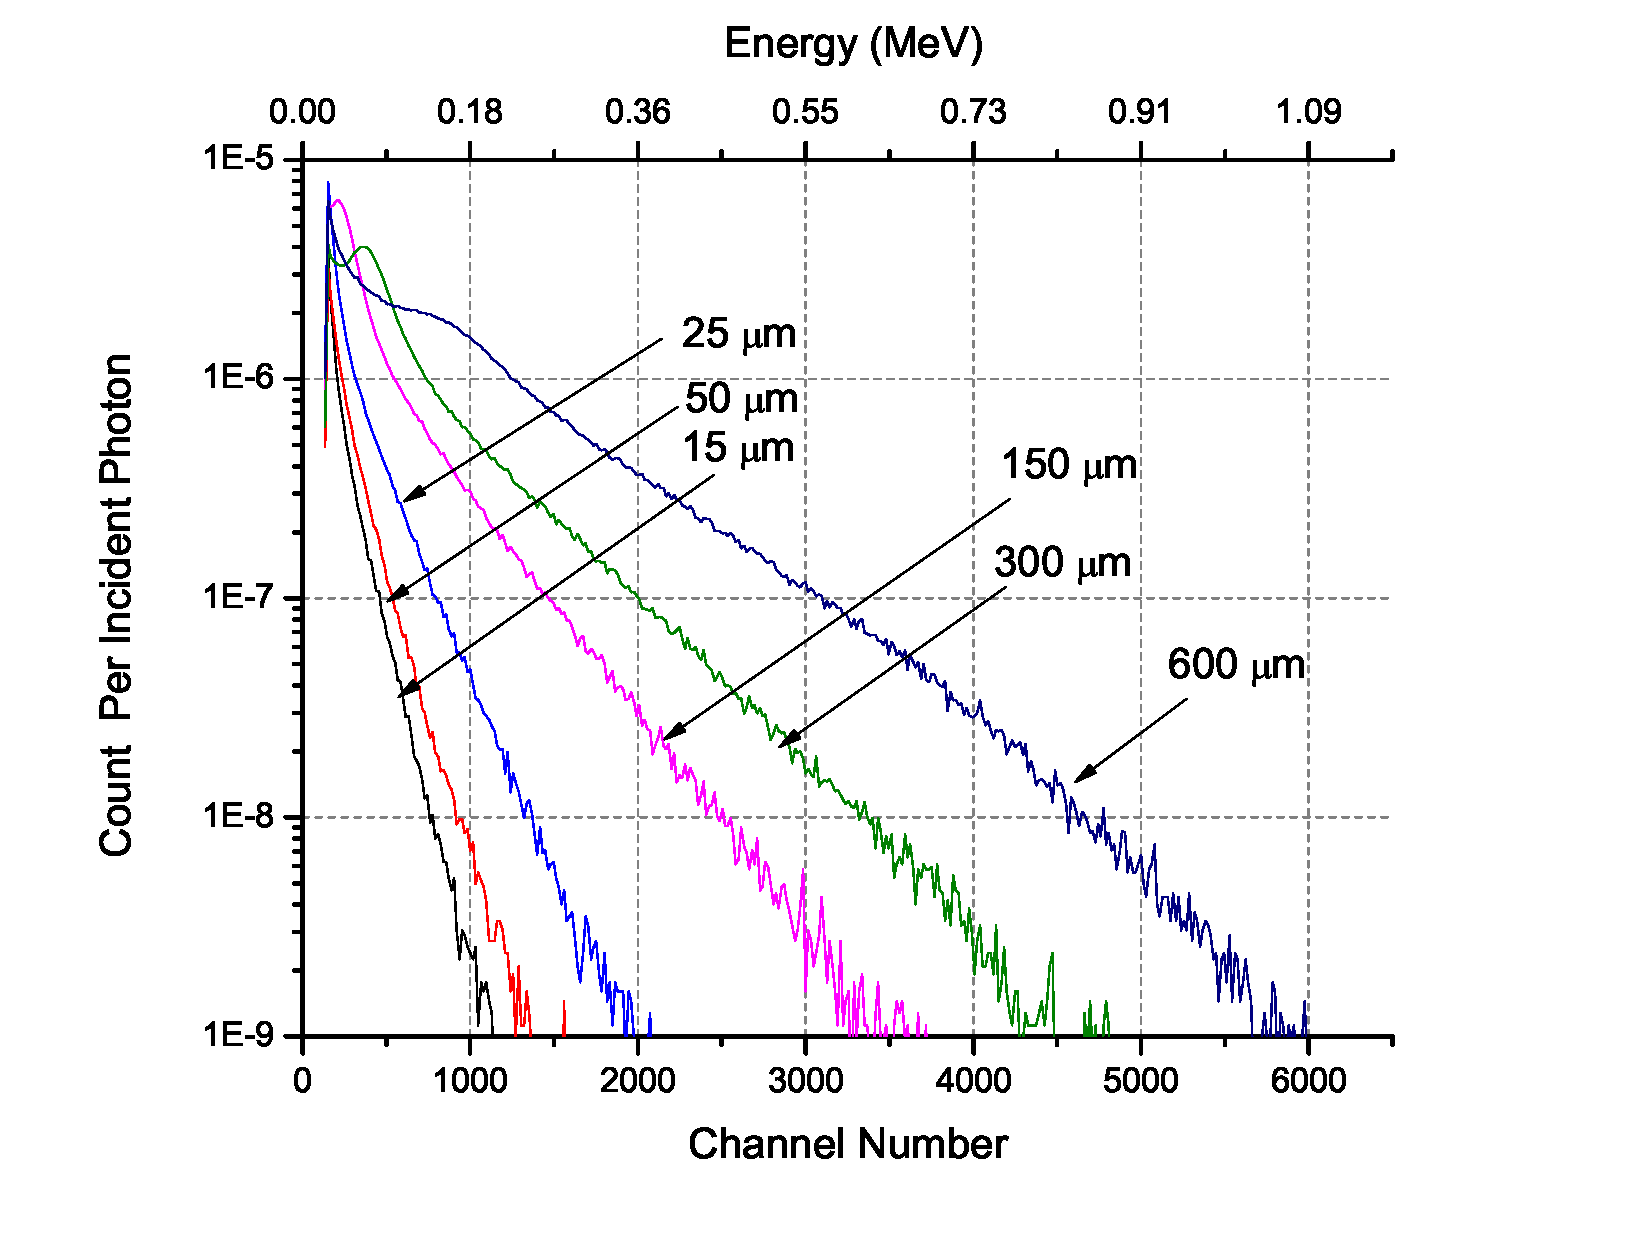
\includegraphics[width=\textwidth]{PS_GammaCR-Binned-FluxNorm_20LiF_5PPO}

      Measured Pulse Height Spectra
    \end{column}
  \end{columns}
\end{frame}
\begin{frame}{Average Light Yield and Average Energy Deposition}
  \begin{columns}
    \begin{column}{0.45\textwidth}
      \centering
      \includegraphics[width=\textwidth]{G4EDep_LightYield_Co60}

		  Gamma (\iso[60]{Co})
    \end{column}
    \begin{column}{0.45\textwidth}
      \centering
      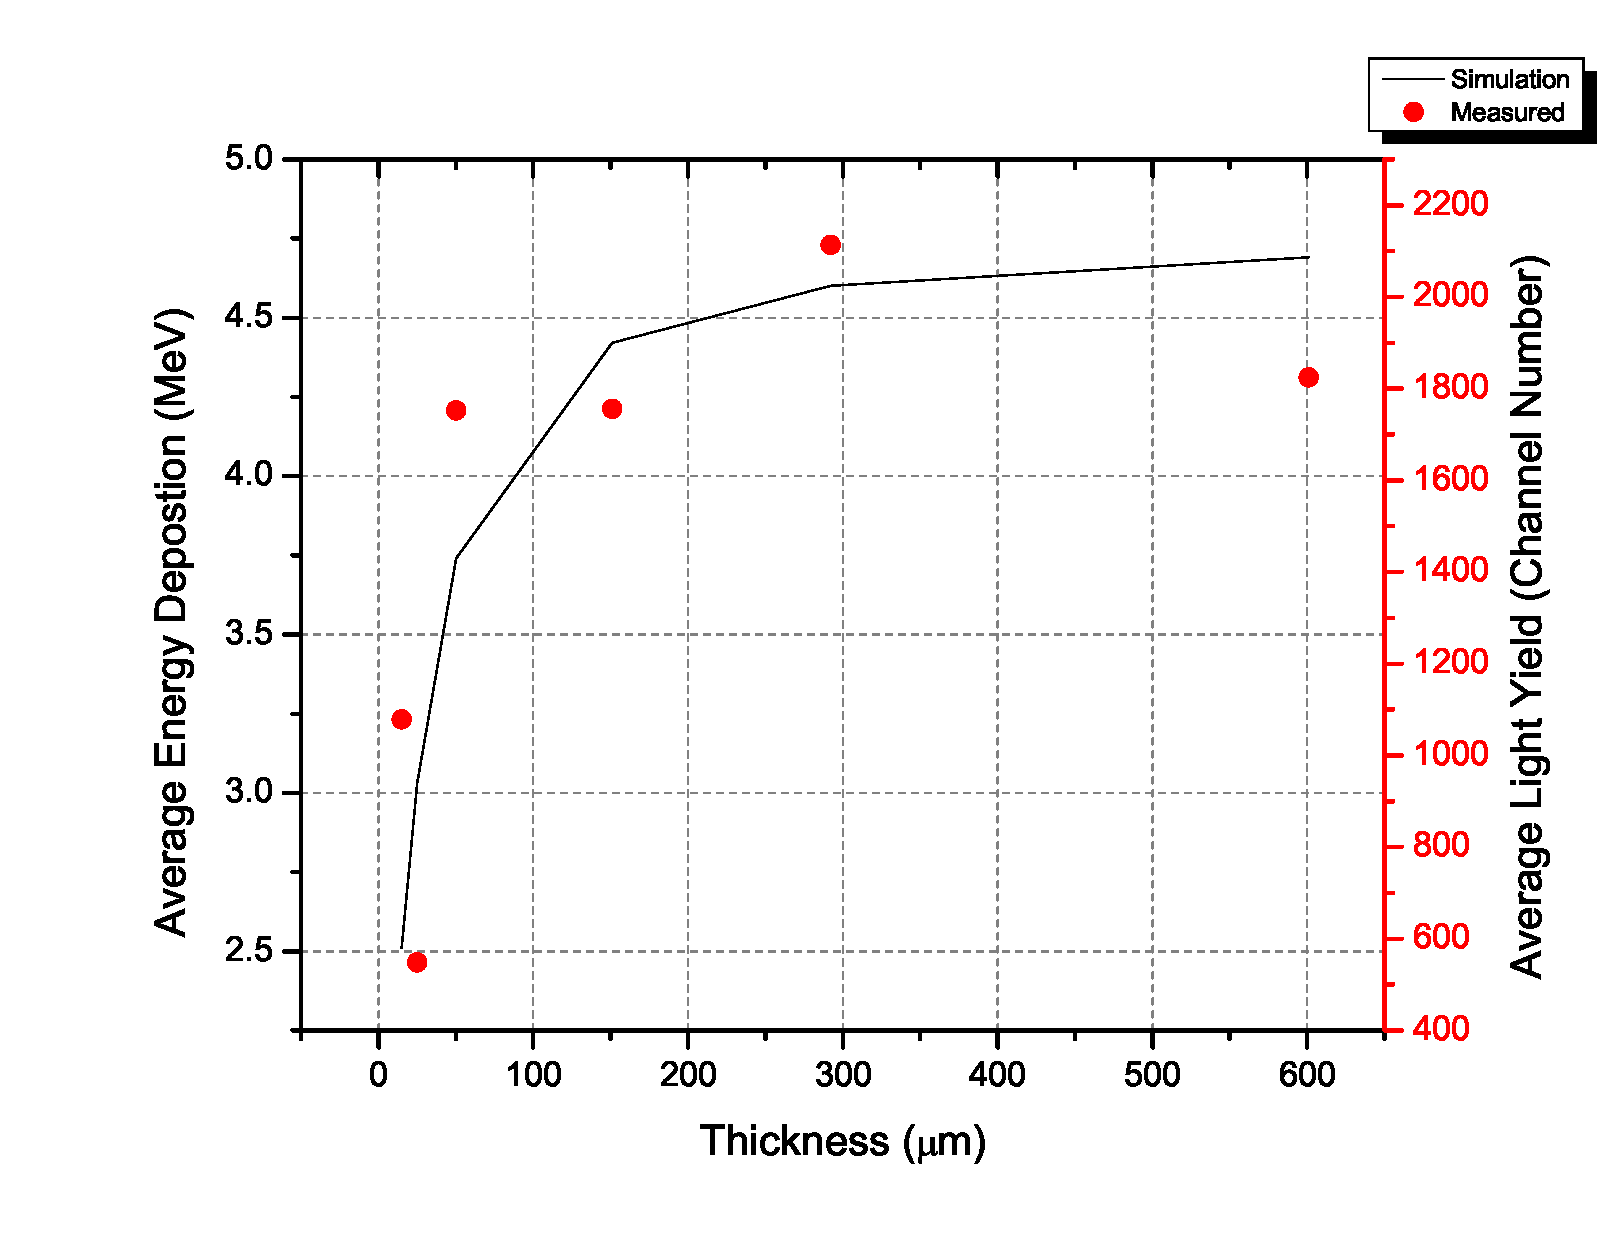
\includegraphics[width=\textwidth]{G4EDep_LightYield_Neutron}

		  Neutrons
    \end{column}
  \end{columns}
\end{frame}
%%%%%%%%%%%%%%%%%%%%%%%%%%%%%%%%%%%%%%%%%%%%%%%%%%%%%%%%%%%%%%%%%%%%%%%%%%
%                                                                        %
%                            CONCLUSIONS                                 %
%                                                                        %
%%%%%%%%%%%%%%%%%%%%%%%%%%%%%%%%%%%%%%%%%%%%%%%%%%%%%%%%%%%%%%%%%%%%%%%%%%
\section{Summary}
\begin{frame}{Summary}
  \begin{itemize}
    \item GEANT4 has the ability to accurately simulate low energy electrons in water
    \item Successfully validated a GEANT4 simulation of the energy deposition of electrons in water
    \begin{itemize}
      \item Improvements in cross sections allow for greater accuracy to be observed
      \item Same spectral shapes are observed
    \end{itemize}
  \end{itemize}
\end{frame}
\begin{frame}{Energy Depostion in thin Polymers}
  \begin{itemize}
    \item Calculated the energy deposition of \iso[60]{Co} photons and neutrons in \SI{15}{\um} to \SI{600}{\um} films
    \item Neutron - gamma discrimination can be enhanced by preferential energy deposition
  \end{itemize}
  \begin{table}[ht]
      \caption{Fractional Energy Deposition for Various Thickness}
    \centering
    \begin{tabular}{c | c c}
    Thickness & Gamma Fraction & Neutron Fraction \\
    \hline
    \hline
    \SI{15}{\um} & 0.010 & 0.531 \\
    \SI{25}{\um} & 0.013 & 0.634 \\
    \SI{50}{\um} & 0.017 & 0.782 \\
    \SI{150}{\um} & 0.032 & 0.927 \\
    \SI{300}{\um} & 0.052 & 0.964 \\
    \SI{600}{\um} & 0.087 & 0.982 \\
    \SI{1}{\mm} & 0.130 & 0.989 \\
    \SI{1}{\cm} & 0.425 & 0.998 \\
    \end{tabular}
    \label{tab:FractionEDep}
  \end{table}
\end{frame}
%%%%%%%%%%%%%%%%%%%%%%%%%%%%%%%%%%%%%%%%%%%%%%%%%%%%%%%%%%%%%%%%%%%%%%%%%%%
\begin{frame}{}
  \centering
  \begin{figure}
    \includegraphics[height=3cm]{PowerTQuestion.png}
  \end{figure}
\end{frame}
%%%%%%%%%%%%%%%%%%%%%%%%%%%%%%%%%%%%%%%%%%%%%%%%%%%%%%%%%%%%%%%%%%%%%%%%%%%
% BILBIOLGRAPHY
\begin{frame}[plain,allowframebreaks]
\frametitle{Works Cited}
	\tiny
  \bibliography{../Zotero}
\end{frame}

\end{document}


